\documentclass[11pt]{memoir}

\def\watermarkloaded{0}

\def\Title{A Wildness of the Heart}
\def\FullTitle{\Title}
\def\AuthorFirst{Madison}
\def\AuthorLast{Scott-Clary}
\def\AuthorFull{\AuthorFirst\ \AuthorLast}
\def\Illustrator{Artist}
\def\IllustratorWeb{www.patreon.com/artist}

\def\Edition{First}
\def\EditionsList{10 9 8 7 6 5 4 3 2 1}
\def\Year{2021}

\def\ISBN{XXX-X-XXXXXX-XX-X}

\def\Publisher{PUBLISHER}
\def\PublisherEmail{publisher@example.com}
\def\PublisherURL{example.com}
\def\PublisherLocation{City, STATE}

%%% Watermark for draft
\usepackage{draftwatermark}
\def\watermarkloaded{1}
\SetWatermarkLightness{0.9}

%

%%% Resets
% memoir defines footruleskip, we want fancyhdr's
\let\footruleskip\undefined
\DisemulatePackage{setspace}

%%% Hyperref warning suppression
% I want math symbols, hyperref complains
% must be before hyperref included
\usepackage{silence}
\WarningFilter[pdftoc]{hyperref}{Token not allowed in a PDF string}
\ActivateWarningFilters[pdftoc]

%%% Package imports not needing expansion
\usepackage{graphicx}
\usepackage{hyperref}
\usepackage{setspace}
\usepackage{xifthen}
\usepackage{xltxtra}
\usepackage{verse}
\usepackage{paracol}
\usepackage{marginnote}
\renewcommand*{\marginnotevadjust}{0.75ex}
\setlength{\columnsep}{0pt}

%%% Headers and page styles
\usepackage[pagestyles]{titlesec}
\usepackage{fancyhdr}
\setlength{\headheight}{15.2pt}

% ourbook style with fancy headers and chapter headings
\fancypagestyle{ourbook}{
  % headers
  \renewcommand{\headrulewidth}{0pt}
  \renewcommand{\printchaptername}{}
  \renewcommand{\chapternamenum}{}
  \renewcommand{\printchapternum}{}
  \renewcommand{\printchaptertitle}[1]{%
  \TitleFont\huge ##1}
  \setsecheadstyle{\TitleFont}
  \renewcommand{\partnamefont}{\DisplayFont\huge}
  \renewcommand{\partnumfont}{\DisplayFont\huge}
  \renewcommand{\parttitlefont}{\DisplayFont\Huge}
  \renewcommand{\chaptername}{}
  \renewcommand{\thechapter}{}
  \setlength{\parskip}{0pt}
  \fancyhf{}
  \fancyhf[FRO,FLE]{\thepage}
  \fancyhf[HRO]{\tiny\DisplayFont\leftmark}
  \fancyhf[HLE]{\tiny\DisplayFont\rightmark}
}

% plain style with only page num
\fancypagestyle{plain}{
  \fancyhf{}
  \renewcommand{\headrulewidth}{0pt}
  \renewcommand{\footrulewidth}{0pt}
  %\fancyhf[FRO,FLE]{\thepage}
}

% single space after periods
\frenchspacing

% Attempt justification at all costs
\sloppy

% Widows and orphans
\widowpenalty=10000
\clubpenalty=10000

% page sizes for trade paperback
\usepackage[
  paperwidth=6in,
  paperheight=9in,
  layoutwidth=6in,
  layoutheight=9in,
  vmargin=0.5in,
  outer=0.5in,
  inner=1.1in,
  includeheadfoot,
  twoside,
  showcrop
]{geometry}
\ifdefined\SetWatermarkHorCenter
  \SetWatermarkHorCenter{3in}
  \SetWatermarkVerCenter{4.5in}
\fi


%%% ToC munging
% Remove ToC header
\renewcommand{\contentsname}{}
\renewcommand{\cftdot}{\small{$\cdot$}}
\renewcommand{\cftchapterdotsep}{3}
\renewcommand{\cftsectiondotsep}{10000}
% start toc at top of page
\renewcommand*\tocheadstart{}{}
\hypersetup{final}

%%% Font
% Uncomment and modify to your font specs

\usepackage{fontspec}
\setmainfont{Gentium Book Basic}
\newfontfamily\TitleFamily{Tom's New Roman}
\newfontface\TitleFont{Tom's New Roman}
\newfontfamily\HeaderFamily{Gentium Basic}
\newfontface\HeaderFont{Gentium Basic}
\newfontface\ChapterFont{Spectral}
\newfontfamily\TocFont{Gentium Basic Bold}
\newfontfamily\SmileyFont{DejaVu Sans}

%%% Title page
\title{\TitleFont{\FullTitle}\\ \vspace{1cm}\large\Subtitle\vfill\null}
\author{\DisplayFont{\AuthorFull}}
\date{}

%%% Section divider
% don't forget to \noindent the line after!
\renewcommand\rule[2]{$\star$}
\newcommand\secdiv{
  \begin{center}
    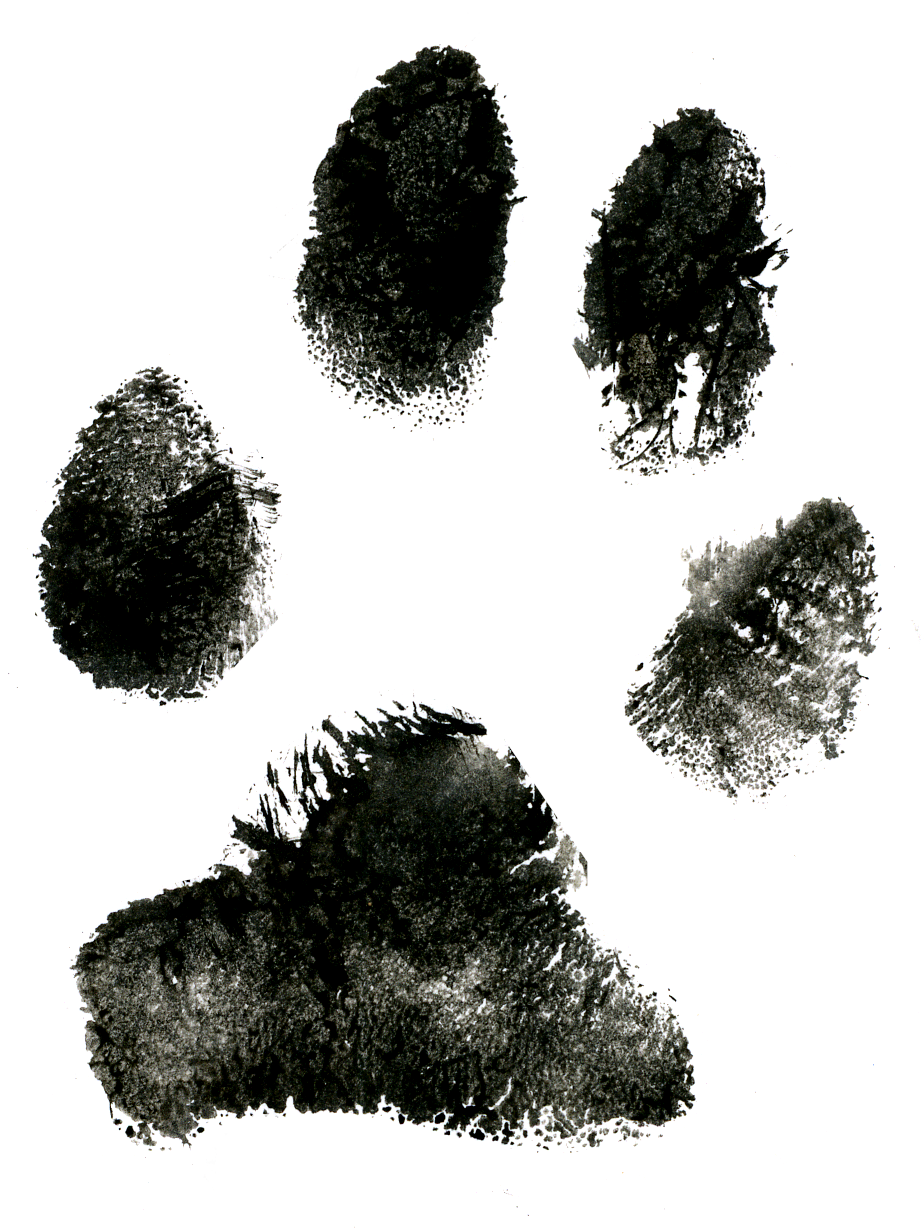
\includegraphics[width=0.5cm]{assets/zpaw.png}
  \end{center}
}

\newcommand\storydiv{
  \begin{center}
    \null
    \vfill
    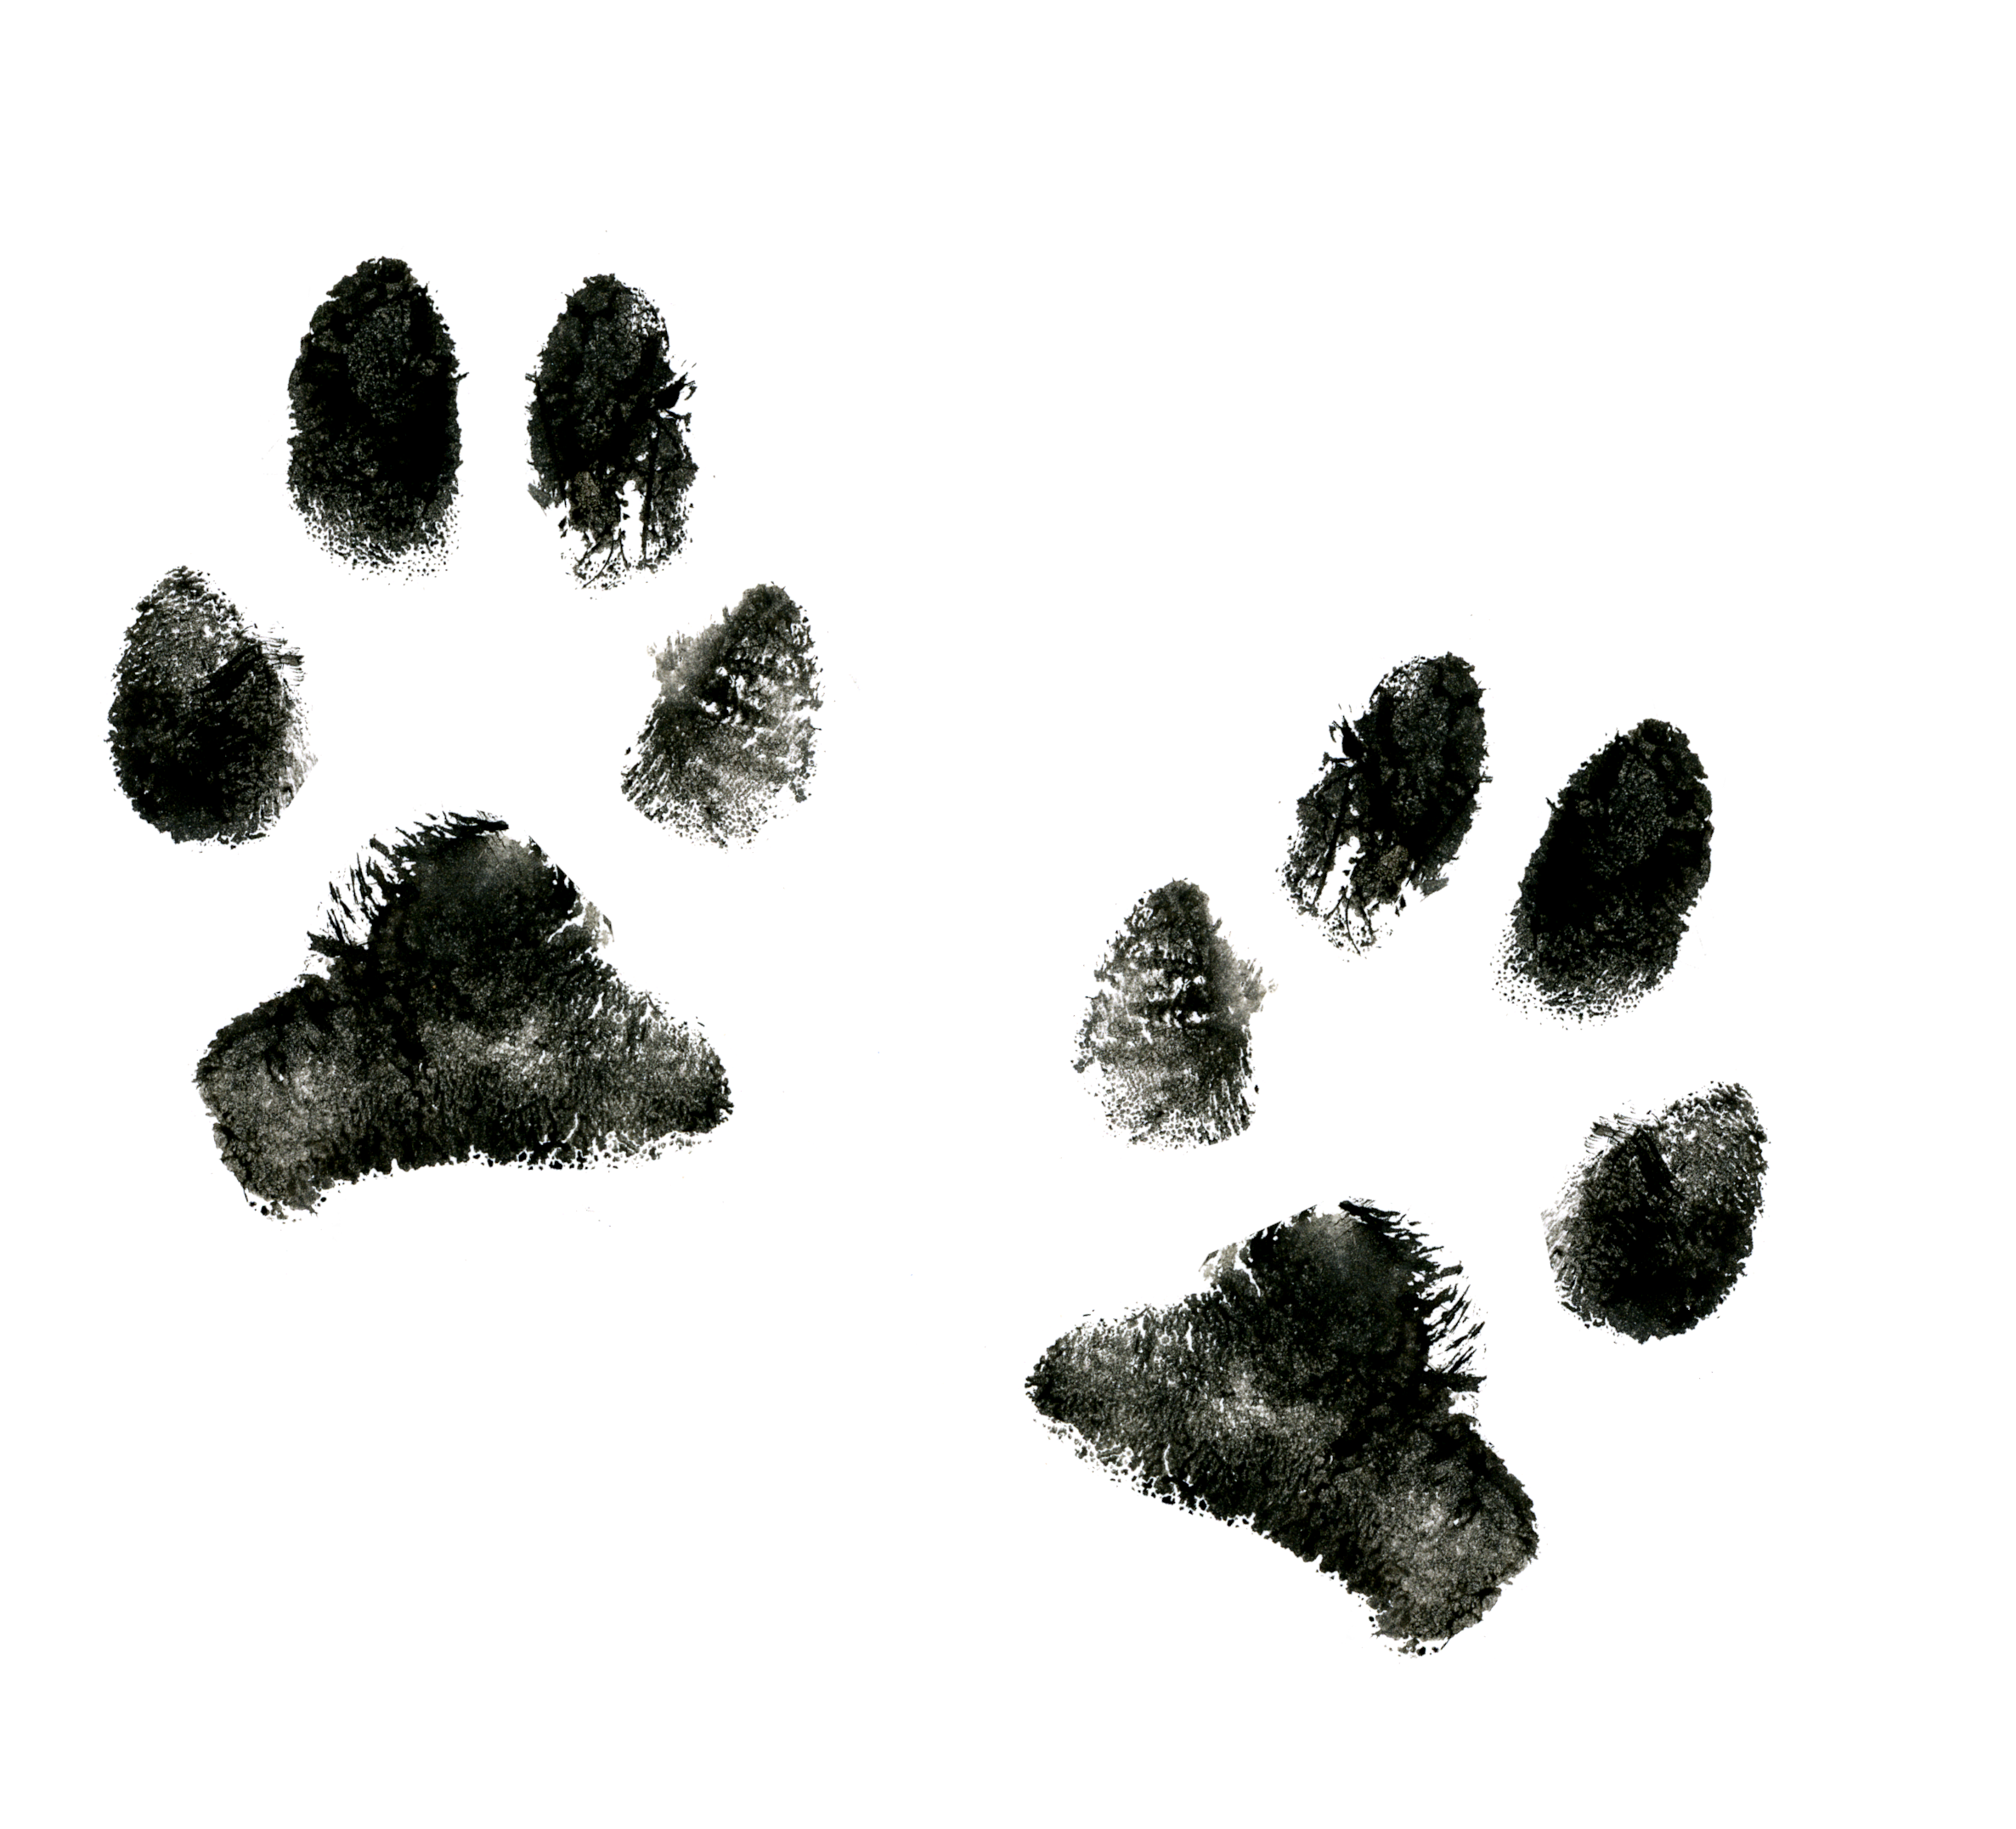
\includegraphics[width=1.7cm]{assets/2zpaw.png}
    \vfill
  \end{center}
}

\hyphenation{
\AuthorFirst
\AuthorLast
\Title
\Subtitle
}


\begin{document}
  \frontmatter

  \thispagestyle{empty}
  \null
  \vfill
  \begin{flushright}
    \DisplayFont Mitzvot
    
    \vspace{1ex}

    {\footnotesize and Selected Letters}
  \end{flushright}
  \vfill
  \cleardoublepage

  \pagestyle{plain}

  \doublespacing

  \begin{flushright}
    \null
    \vfill
    {\Huge\DisplayFont Mitzvot}

    \vspace{1ex}

    {\Large\DisplayFont and Selected Letters}

    {\DisplayFont Post-Self book IV}

    \vfill

    {\Large\DisplayFont Madison Scott-Clary}
  \end{flushright}
  \thispagestyle{empty}

  \newpage

  \singlespacing
\thispagestyle{empty}
\begin{center}
    \noindent {\DisplayFont Also by Madison Scott-Clary}
    \TitleFamily

    \vspace{2ex}

    \emph{Arcana — A Tarot Anthology}, ed.

    \vspace{1ex}

    \emph{Rum and Coke — Three Short Stories from a Furry Convention}

    \vspace{1ex}

    \emph{Eigengrau — Poems 2015-2020}

    \vspace{1ex}

    \emph{ally}

    \vspace{2ex}
    
    \textbf{Post-Self}

    I. \emph{Qoheleth}

    II. \emph{Toledot}

    III. \emph{Nevi'im}

    IV. \emph{Mitzvot}

    \vspace{2ex}

    \textbf{Sawtooth}

    \emph{Restless Town}

    \emph{A Wildness of the Heart}

    \vspace{2em}

    Learn more at \emph{makyo.ink/publications}
\end{center}
\vfill
\singlespacing
{\small\parindent0pt\parskip5pt
\noindent Copyright \copyright\ 2020, Madison Scott-Clary. This work is licensed under the Creative Commons Attribution 4.0 International License. To view a copy of this license, visit \mbox{\emph{creativecommons.org/licenses/by/4.0/}} or send a letter to Creative Commons, PO Box 1866, Mountain View, CA

\vspace{1ex}

ISBN: \ISBN

\vspace{1ex}

\textit{Nevi'im}

\vspace{1ex}

Cover \copyright\ Iris Jay, 2022 --- irisjay.net

\vspace{1ex}

%\textit{This digital edition has been posted to Internet Archive and OpenLibrary by the author.}

\Edition\ Edition, \Year. All rights reserved.

\vspace{1ex}

This book uses the fonts Gentium Book Basic, {\DisplayFont Gotu} and {\TitleFont Linux Biolinum O} and was typeset with {\usefont{OT1}{cmr}{m}{n}\XeLaTeX}.

%Printed in the United States of America\\
%\EditionsList
}%\parindent0pt

\clearpage


  \tableofcontents*
  \newpage
  \null
  \cleardoublepage

  %\onehalfspacing
  %\doublespacing

  % \null

\vfill

\noindent \textbf{Content Warning:} These stories contain descriptions of sex and sexuality. \emph{How Many} contains explicit description of mental health issues. \emph{Again} contains drug use.


  \mainmatter

  \pagestyle{ourbook}

  \cleardoublepage
  \null
  \thispagestyle{empty}
  \vfill
  \begin{quote}
    \small
    \emph{When you make a vow to your God~{\HebFont יהוה}\,, do not put off fulfilling it, for your God~{\HebFont יהוה} will require it of you, and you will have incurred guilt; whereas you incur no guilt if you refrain from vowing. You must fulfill what has crossed your lips and perform what you have voluntarily vowed to your God~{\HebFont יהוה}\,, having made the promise with your own mouth.}

    --- Deuteronomy 23:22--24
  \end{quote}
  \vfill

  \part*{Mitzvot}
  \addcontentsline{toc}{part}{Mitzvot}

  \hypertarget{true-name-2124}{%
\chapter{True Name—2124}\label{true-name-2124}}

The next meeting spot for the Council of Eight was in a rooftop bar. However, given that that rooftop bar was in the midst of a block of apartment buildings and vertical malls that had built with shared walls, such that there was a cubic half-mile of stair-climbing, elevator rides---down as well as up---and trestles that bridged buildings of lower height than higher ones, it was more adventure getting to the venue than the meeting itself promised.

Still, The Only Time I Know My True Name Is When I Dream climbed.

The apartment buildings ranged from serviceable to gutted, and more than one time, she had to step carefully through a path covered in rubble. She could not decipher whether this was due to abandoned renovations, some unknown battle, or the simple degradations of time.

The malls offered different dichotomies. Some of them were sparkling new with speakers that whispered to her in Mandarin and lights that shouted in her face, while others played placid muzak through halls lit only by emergency lights, darkened storefronts yawning onto scuffed and over-waxed parquet floors.

She wondered who it was that had owned this sim, what collective it was that had decided to mash all the best and worst multiple clashing centuries worth of Kowloon Walled City and the North American Central Corridor.

And then, the rooftop bar. Despite no vehicle entrance to the complex, this was situated on the top level of what appeared to be a car park straight out of a mid-western American airport, complete with one or two of those vehicles that seemed perpetually parked, ones that had lingered for months or years, accruing a parking debt of thousands, tens of thousands of dollars.

The bar itself was a pop-up affair, with walls and ceiling of corrugated plastic held together with rivets and tape, a bar-top that was a few two-by-eights set across a trestle, fronted with further corrugated plastic to keep the patrons from kicking fridges or sinks out of alignment.

The drinks: early 2100s hipster bullshit, all intensely sweet or riddled with smoke-scented fizzy water or long strips of seaweed or clams within the ice cubes, steadily making the drink more and more savory over time.

True Name found it all confusing and jarring.

She liked it immediately.

Debarre was already at one of the tables---similarly cobbled together---sipping something that seemed to be all foam. He waved to her as she entered, and she waved back, heading to the bar to pick up one of those seaweed concoctions before joining him.

``That looks fucking gross, Sasha.''

She laughed and shrugged. ``I am True Name, but yes, it really does. If we are going to meet in a place that gives me a headache to walk through, it is probably best that I get something with\ldots protein? Is that how this works?''

``Uh, sorry. Yeah. True Name.'' The weasel splayed his ears and averted his eyes. ``Can we talk about that sometime?''

``Yes, but probably as Michelle, if that is okay.''

``Why?''

``She is\ldots closer to it than I am.''

Debarre gripped his glass more tightly and twisted sideways to swing his leg over the bench and straddle it. ``Yeah, I don't get it. Before everyone else gets here, can you at least give me a sentence or two?''

``When she forked, when I\ldots became me, she decided not to fork that part of her that suffers if that is the right word.'' True Name frowned. ``Already we are drifting further apart. The species remains, the appearance and the speech patterns remain, the \emph{mind} remains, but not that part of her that is so split. I am me, I am templated off of Sasha, because being both Michelle and Sasha at the same time was no longer tolerable.''

He shrugged, still staring down into his drink. ``I can't speak to that, I guess. But why Aw--''

True Name slammed her glass down on the table a bit harder than intended, some of the drink spilling over her hand. ``Do not say that fucking name.''

The weasel jumped at the sudden intensity, and when he recovered, he finally met her gaze. His expression softened from fear and anger to a tired bleakness. That moment drew out for a long few seconds of quiet and seething sadness. He reached for a napkin from the dispenser at the end of the table and handed it to her. ``Here.''

She hesitated, mastered a surge of unnamed emotion, and accepted the napkin to wipe the sticky drink from her paw and then, on realizing that she was crying, the tears from her face. ``Sorry, I am just\ldots{}''

``We'll talk.'' He reached over and gave her dry paw a squeeze in his own. ``Michelle and I will. There's something I'm missing here is all, and I want to figure out why more than what.''

True Name hid her muzzle in her drink and pretended to take a sip until she was sure she wouldn't slur her words when she spoke. ``Thank you. She is open to messages still, I will let you two work it out. For now, I need to focus on the meeting. Jonas and Zeke are here.''

Looking over his shoulder, Debarre nodded and turned to sit on the bench to face her again, leaving room for the other two. Jonas settled next to True Name so that they could give their speech together when the time came, and Zeke, that shifting bundle of rags and grime slid onto the bench beside Debarre.

``Good afternoon,'' the almost-face within the bundle rasped.

Jonas grinned. ``It's morning, isn't it?''

A pseudopod that may have been a hand waved the comment away. ``Time has lost all meaning. I seem to have forgotten how to sleep, these days.''

``You need a vacation like Michelle.''

There was a low rattle from the rags, and True Name imagined that must be Zeke's laughter. ``Don't tempt me. I don't have the funds to fork, so you'd be down to seven.''

``Why \emph{did} you make it so expensive?'' Jonas elbowed True Name in the side.

She held up her paws defensively and laughed. ``I did not. The price is tied to system capacity.''

``The laws of physics were a mistake and reputation is a lie.''

``It is the best limiting factor that we have that is not a complete fabrication, at the moment.''

``I rather miss coins.''

``My dad used to collect coins, you know.''

And so on, until the table was full and the cone of silence fell.

``Sasha? Uh\ldots True Name. Jonas?'' one of the well-dressed triad asked.

``Right,'' Jonas said, setting his drink down. ``The bill. Things are progressing slowly, as they always do, but it sounds like they might start picking up steam shortly. Our main contact on the DDR side, one Yared Zerezghi based out of the Northeast African Coalition, says that some of the governments are starting to take interest in the bill, which could work to our advantage. Having it just be a direct vote would mean that we would have far, far more representatives to convince, since that'd mean essentially everyone on the DDR. The more governments in play, the more the role of the DDR shrinks.''

``How does that even begin to help? Aren't they super stodgy?'' Debarre asked.

``They can be,'' Jonas hedged. ``But if we can form contacts with each of them, we can argue our case directly. Yared might be the one to give us a good in for the NEAC, and I still have some Western Fed contacts.''

``Anyone for the S-R Bloc or anywhere in SEAPAC? Middle east? India?''

The trio of suits raised their hands. ``S-R Bloc. We don't know any of the oligarchs directly, but we had some big money interests of our own.''

``Israel,'' Zeke said, then laughed at the awkward silence that followed. The trio frowned. ``Sorry, nothing to be done there.''

``And SEAPAC?''

user11824 shrugged. ``I was a nobody, but I was a Maori nobody.''

``You had enough to upload. That has to count for something, doesn't it?''

He shrugged again.

``We will take all the help we can get,'' True Name said. ``Even from nobodies.''

``Alright, I'll poke mom.''

Zeke nodded to True Name. ``What's your take on the situation?''

She stirred her drink to buy herself some time to think. ``I think it is leaning our way. One of the big arguments remains speciation, but Yared's turning that into a pro-rights argument instead of a neutral- or anti-rights one. His voice is getting louder, too. It sounds like he is getting a lot more upvotes on his posts than before.''

``That's good.''

True Name nodded. ``I think so. He is not the biggest voice on the issue yet, but it sounds like he is probably in the top three.''

``You said he's NEAC, right?''

``Yeah, Addis Ababa,'' Jonas said. ``Not exactly the seat of power, but I guess not everything has to be Cairo. Sounds like we have a good mix, at least. No one from South America?''

Everyone shook their heads.

``I suppose that's alright. They're a big enough voice in Western Fed, but they're still in the shadow government side of things. They don't even have the shadow minister of System affairs.''

``Who does?''

``Lithuania.''

One of the suits laughed, and Debarre looked blank.

``Politics,'' Jonas said, grinning lopsidedly.

``If you say so.''

After a moment's silence, Zeke rasped, ``So what are our next steps?''

``Let's all talk to our respective interests---Zeke too---and we'll meet again soon. True Name and I will keep working with Yared and guide as best we can from our side. Speaking of, though, any thoughts on the speciation topic?''

Six sets of eyes flitted between Debarre and True Name, between weasel and skunk, then the whole council laughed.

``I don't give a shit,'' user11824 said. ``But if your Yared guy can twist that argument against the opposition, then that's just one more tool, isn't it?''

``We aren't seeing that,'' the man in the suit spoke up. ``Two thirds of our power structure still think child restrictions are a good enough idea that those laws have bled into Russia. I'm pretty sure they see speciation as a positive. What better way to help in population control?''

One of his companions shrugged, ``I wouldn't be surprised if they started putting limitations on uploading by gender, but that is a separate topic.''

``Zeke?''

The pile of rags shifted in a shrug.

``Debarre? True Name? Anything you can leverage?''

The weasel laughed. ``I mean, if you want to point to us as an example to push that along, and Yared's tack seems to be working, go for it.''

``Alright. It's something you can suggest to your respective interests if you think it'll help. We'll reevaluate next meeting. Anything else on the agenda?''

Everyone shook their heads, then lifted their glasses to a toast. The cone of silence dropped.

``Well, then, you are all free to stick around or go if you want,'' True Name said. ``I am going to stay and get well and truly plastered.''


  \chapter*{Snippets}
  ``True Name,'' May said, interrupting the other skunk's tirade. ``Wait.''

Wrong footed, True Name frowned. ``What? Why? I do not--''

May held up her paw, a brief glance at the ceiling hinting at a sensorium message elsewhere.

Ioan frowned as well. Intuition told him the discussion they'd had earlier had gone beyond the hypothetical. ``May, are you sure--''

True Name jolted upright in her seat on the couch. ``What the fuck is--''

``Accept it,'' May said, and ey could see the force of her gaze boring into her cocladist. ``You must do this. You have to.''

Her face contorting with the strain of holding what must be a very large impending merge at bay without either remembering or forgetting it, True Name gasped. ``May\ldots{} May Then\ldots{} Why\ldots{}''

Eir partner's expression softened. ``Please, my dear. I think you need this. I think we all need this, if we are to move forward.''

The skunk nodded shakily, attempted a dry swallow, and then let the merge of End Waking's centuries of memories crash into her.

The change was immediate and more dramatic than ey'd expected. Ey had been expecting a shell-shocked look and maybe a few minutes of silence, but instead True Name's expression melted into a glazed, nearly stroke-like stupor. The glass of water she'd been clutching at but had yet to drink tumbled to the floor and, as all her muscles gave out at once, she began to slide off the couch.

``Shit. Shit! Ioan!'' May shouted.

Ey was already on eir feet and halfway around the table, thankfully in time to catch the skunk before she slid down into the pool of water on the floor. Ey managed to get eir arms under hers enough to hoist her up into the couch again while May ducked around to lift her feet so that they could lay her out on her back.

They both stared at the limp True Name.

``Fuck,'' eir partner murmured.

``What just happened?''

``One second,'' she said, waving away the spilled water so that she could kneel by her down-tree instance. There was a moment's hesitation before she brushed some of the skunk's longer head fur away from her face. ``Can you close your eyes?''

When True Name didn't respond, didn't move, May gently brushed her paw down to close them for her.

After lingering another moment, she stood slowly, took Ioan's hand in her paw and led em to the balcony. As soon as the door shut behind them, she burst into tears.

Ey guided her carefully to the bench swing to sit her down, letting her cry herself out against eir shoulder.

``I am sorry, my dear,'' she said when she could speak again at last. ``Really, truly sorry.''

Ey shook eir head, kissing her between the ears. ``You don't need to apologize to me. I'm more confused than anything. Was that your and End Waking's plan?''

She pressed closer to em. ``That was him merging back down, yes. I did not expect that, though,'' she said, and ey could hear that she was on the verge of crying once more. ``I never intended to hurt her.''

``Can you explain what happened, at least?''

She nodded, swallowing down that wave of tears as best she could. ``We are good at forking and merging. Very, \emph{very} good at it. I am pretty sure you know that, though.''

``Did something go wrong, then?''

``End Waking has not merged down in nearly two centuries. He has diverged quite far in that time, as is to be expected, which means the potential for conflicts.''

Eir frown deepened. Ey thought ey could tell where this was going. ``Aren't those usually just when memories don't line up, though?''

May gave the barest hint of a shrug against em. ``You have met her, and you have met him. Their viewpoints are almost diametrically opposed, yes?''

Ey nodded.

``Viewpoints are built atop a collection of memories. That they can share so many memories and yet have such different outlooks on the world and their actions is a subtler, but trickier sort of merge conflict.'' She paused, took a deep breath, then continued slowly. ``I pressed her to accept because I knew that she would accept the merge as smoothly as she always does if there was external pressure. She merged blithely and took on two hundred years of End Waking all at once. All of his memories. All of his penitence. All of his loathing for what he did, what she was so proud of.''

``And it was too much?'' ey asked.

Her face screwed up again as she nodded. ``I nuh-never wanted t-to hur-hurt her,'' May stammered as the tears started to flow once more.

Ey got eir arms around her again and held her close. A quick glance through the windows showed that True Name still lay on the couch, breathing shallowly.

``May, I want to ask you something,'' ey said, once she had calmed down some. ``And\ldots well, I think it'll probably make you cry again, but I want to make sure we stay open about this. I'm really not asking this to take a jab at you. Is that okay?''

She whined quietly, but nodded all the same.

Ey took a deep breath, keeping eir voice as gentle as ey could. ``I'm not upset with you, but I need to know since this is just getting weirder and weirder. Are you sure you didn't want to hurt her?''

There was a long silence before she replied, and ey could tell she spent much of it counting her breaths, one of the exercises that had worked best to ground her. At least she counted as best she could between sniffles.

``I think,'' she started, then cleared her throat. ``I know a part of me was acting out of vengeance.''

Ey nodded. ``We talked about that, yeah.''

``Right. I think that part was hoping that it would be a rough merge to knock her down a peg, yes,'' she said, then let out a shaky sigh. ``I did not think it would be this bad, though. I am really sorry, Ioan. I want to be a good person.''

Hugging her tightly to em, ey said, ``It's okay, May. You \emph{are} a good person, promise. Just that even good people feel resentment.''

She nodded, fell back into breathing exercises.

``And I believe you when you say you didn't want to hurt her. Both those--''

She elbowed em in the side. ``Right, yes, yes. Both can be true at once. You know we have the same therapist, right? She says the same things to me.''

Ey smiled, pleased to hear the humor in her voice. ``Sorry, May.''

She wormed her arms around em to give a tight squeeze. ``It is alright. You are just a nerd. Both of those things can be true, too.'' After a moment's hesitation, she asked more quietly, ``Can you see her? Is she okay?''

``She's rolled onto her side. Still breathing pretty quick.''

May nodded. ``Let us get back in and check on her, then. We may want to get her into bed. Being comfortable can make it easier.''

(They do, ey carries her, May stays by her side, Ioan leaves so she can apologize in private)

\begin{center}\rule{0.5\linewidth}{0.5pt}\end{center}

  In the most stunning display of forking ey'd ever seen, True Name began to change.

Ioan had seen eir share of Dear's exhibitions, not to mention those of other instance artists the fox had introduced em to along the way, and the forking involved in all of them had been perfect. They were well rehearsed dances of duplication that told a story.

However, they were, whether by virtue of being related to Dear or by the art itself, fanciful. The duplication was supposed to evoke a sense of magic, of wonder (or the closely related terror).

In eir own work in theatre, both as an actor and as a playwright, ey'd found use for forking within a story that had remained more grounded, more tied to day to day life, and those performances had seen a success of their own through May and A Finger Pointing's guidance.

The Odists as a whole were more familiar and comfortable with forking than anyone ey'd ever met, even among the most dispersionista of dispersionista clades. Both May and Dear navigated that aspect of their lives with a grace ey could only dream of. Even the explosions of foxes or skunks during times of excitement were well done.

This, though, went beyond that.

As they stood watching, True Name began to change. She worked with a singular sense of purpose that left no doubt as to what she was doing. An instance flickered into being before herself and watched with a critical eye as skunk after skunk blinked into existence. Each one bore some slight change from their immediate down-tree instance. Sometimes an array of skunks would wind up in a line before that observing instance, which would nod at one or the other in approval to leave the other to quit. And when a change was accepted, the down-tree instance would quit.

This smooth modification of form was in and of itself impressive for how naturally she began to change — not only did the instance watching have to keep track of what change was happening and what would come next, but so did those doing the actual changing; they all had to be on the same page — but what left em truly impressed was the speed. She began her work with about one fork per second, but before long the changes ramped up to four a second. Five. Nearly ten changes per second of forks flickering into and out of existence, all while the orchestrating instance watched, her eyes flicking this way and that across them.

And then, it was over.

The result was a skunk slightly shorter than True Name had stood, though still a few centimeters taller than May. She was heavier, as well, with a curve to the hips and belly that was familiar to em from eir partner, but unlike May, this softness was more\ldots well, natural wasn't quite the right term, but where May's weight seemed to be designed to add a sense of both harmlessness and comfort to her form, this new form of True Name simply looked like a pudgy thirty-something who had settled into a comfortable weight long ago and never bothered to change.

Her face had shifted as well, becoming plainer in ways ey couldn't quite explain. Where True Name had always had some aspect of larger-than-life about her, she now just looked\ldots normal. Still a furry, still living in that form that was more comfortable to her than humanity, but normal.

Most striking, though was the pattern of fur. While much of it was covered, now, ey'd seen the way it had shifted during the process. Gone were the stripes, the ones ey had grown to love on May, replaced now with a set of white splotches in the black of her fur. The pattern was what was so eye-catching, however: the patches seemed to travel in a few uneven lines down over her back and sides, one of them showing a hint of a whorl, another a slight zigzag as it ran from her spine to her side, and others that were almost round spots. This pattern seemed to be mirrored along her spine, leading to a pleasant symmetry. A quick query of the perisystem infrastructure told em that there was indeed a spotted variety of skunk, described much as ey had seen.

Gone were the stripes. Gone, also, were the slacks and blouse, traded in for a linen tunic and a pair of loose-fitting trousers of the type ey had always associated with southeast Asian fishers.

When ey was finally able to tear eir eyes away, ey saw that every Odist in the room had picked up expressions that verged from taken aback to startled and angry. May, for her part, looked startled, yes, but also excited.

``May, what--''

``One moment, my dear,'' she said, then turned to face this new True Name with a grin. ``Will there be a change of name?''

``There has to be,'' Jonas said. While he lacked the context for whatever had surprised her cocladists, even he sounded impressed by the display. ``I won't let you leave as True Name.'' ((Probably needs expansion))

The skunk bowed. ``You may call me Sasha.''

Ioan didn't know what ey expected from the room, but pandemonium wasn't it. May was bouncing on her feet and clapping her paws. End Waking was grinning and shaking his head. Jonas had simply burst out laughing.

All of the rest of the Odists, however, were shouting. None of them looked pleased.

``Not Sasha of the Ode clade, just Sasha,'' she said. ``I will not relinquish the form, just as I will not relinquish the past, but if you want me out this badly, so be it. I rescind my membership in the clade.''

``\emph{That} name is unacceptable,'' When I Dream hollered. ``No.~You will pick something else.''

``No, I will not.''

``Shut the fuck up, When I Dream,'' Jonas said mildly. ``All of you, shut the fuck up.'' He turned to Sasha and grinned. ``You always were a little snot. You want to be Sasha? You want to dive back into mediocrity and wear your weakness like a badge? Please, by all means, be my guest. Beg for pity again. Hunt down all your little friends who kept you feeling just bad enough that they could baby you without letting you think you were their plaything. Go. Be Sasha. Live your silly little life. ((way more, and angrier))

``And you,'' he growled, jabbing a finger toward Ioan. ``Write your little story. That's what you're here for, isn't it? Write your little romance and fuck your little girlfriend and put on your little plays.''

May rolled her eyes.

``Get out. All of you.''

All through Jonas's tirade, Sasha wore a slight smile. It wasn't beatific, wasn't enlightened. She simply looked present. She looked confident in herself in some more earnest way. When it was clear that he was finished, she bowed politely.

``See you around?''

``Fuck off.''

She laughed and reached out to take Ioan's hand in eir paw, then they stepped back home, followed closely by May holding End Waking's paw.

There was a long moment of silence in the living room, then Ioan let out a ragged, pent-up breath, eir shoulders sagging. ``Can someone tell me what the fuck just happened?''

``Sasha found the one thing she could have done to piss off Jonas,'' May said, looking at her appraisingly. ``He went in thinking he'd take everything from her and left with no wind in his sails. Well done, my dear.''

Sasha beamed and bowed with a flourish

``And you knew this?'' ey asked.

She shook her head. ``I saw her unwind all of the changes from the last centuries--''

``All the way back to Praiseworthy's suggestions before Secession,'' the other skunk said proudly.

``--and other than the spotted skunk thing, she looks just like\ldots well, Sasha. Nice touch, by the way.''

``I do not think I could have gotten away with staying that similar, but yes, I am back to the me of\ldots{} Shit, when did I make Sasha like this? 2110?''

Ioan shook eir head, dizzy. ``This is what you looked like before uploading?''

``What my — \emph{our} — av looked like, yes, all except the change to a spotted skunk. They always felt too flashy, back then, and I just wanted to look like myself offline except a furry. Completely unremarkable and a species no one likes.''

``It was the outfit that did it,'' End Waking said. ``It always was our favorite, but for some reason, we never brought it with us to the System.''

Sasha nodded.

``I am proud of you, Sasha,'' he continued. ``I do not yet know why I feel compelled to say that, but I am proud of it. You have much to make up for, your own penance yet to serve, but that you have done this at all is good step forward.''

Ioan sighed and pulled a chair out from the dining table and sat down heavily. ``You all are nuts.''

The three skunks laughed.

``So,'' ey said, organizing eir thoughts out loud. ``May and End Waking merged down and you\ldots{} I guess feel more complete with those identities? Enough to head back to who you were before the clade began, I mean. Is that even possible?''

``It is not a statement of reality, my dear. I cannot reintegrate those aspects of myself that are not up-tree from me, and even if I could, there are those who no longer exist or who have left Lagrange,'' she said, that slight smile growing. ``It is a statement of hope, perhaps, or a desire for completion. It is an understanding of the ways in which I fall short expressed in my very name. Will this sense of a more complete life last? Perhaps. It will certainly not always feel good, and will at some point cease feeling new, but I plan on owning it for as long as I am able.''

``And how is it that this pisses of Jonas?'' Ey snorted. ``He certainly sounded pissed.''

Sasha pulled out the chair across from Ioan and sat down, followed shortly by May and End Waking to either side of em. It was strange to see so many smiles around the table, still strange to see May so happy around her down-tree instance — at least logistically, if no longer spiritually — and stranger still to see End Waking even near her.

``What Jonas was suspecting was for me to remain True Name in everything except form and name,'' she said. ``He was expecting someone deeply cowed by his political genius. And do not underestimate him, he \emph{is} still a genius. He felt that he had won his spot as rightful leader of Lagrange, if such a thing can even be said to exist. He had beaten me down and left me either unable to continue or unwilling to try.''

Ioan jumped at a brief sensorium ping, a request to enter, followed shortly by Debarre popping into existence behind May, who had apparently admitted him. ``What was so urgent that you pulled me out of the woods and\ldots{}'' he trailed off, squinting at this new skunk at the table. ``Who\ldots but you're\ldots what?''

``Debarre,'' Sasha said, bowing her head. ``A pleasure to see you.''

The weasel said nothing, looking stunned.

``This is-- was Tr--''

``Sasha. I am Sasha, and I was her as well,'' she said, voice gentle but insistent enough to stop Ioan from continuing.

He stepped back a half pace, crouching as though to flee. ``Sasha\ldots? What the fuck?''

Ioan, still feeling eir head spinning from so much happening so quickly, tried to pin down eir open question in eir mind while still watching the exchange intently.

``I am not what I was, Debarre. I am not True Name. I am not May Then My Name or End Waking.'' She hesitated, then continued, ``I am not even the Sasha you remember, but I am, I think, closer to being her than any of the Ode clade is currently.''

``Bullshit,'' he growled. ``If there's even a little bit of True Name in you, you can't be her. If you're even the slightest bit her I'm fucking out of here.''

``Wait, my dear,'' End Waking said. ``Please stay.''

Debarre hesitated.

``If I am still here, do you not think that I agree with her? At least to a large enough extent to trust her?''

The weasel straightened up and, when May waved a fifth chair into existence beside End Waking, he slowly sat down, resting only on the edge as though still ready to bolt. ``I'll listen, but this had better be good.''

Sasha bowed, sitting quietly while May caught him up on the events of the past few days, letting the other three of them interject with corrections and confirmations. Throughout, Debarre waited, and while he didn't relax fully, by the end of the discussion, he was at least sitting all the way back in his chair.

``So you're now this new Sasha,'' he said slowly. ``I'll buy that, though you still make me nervous.''

She laughed. ``Do not worry, my dear. I make myself nervous.''

At the affectionate \emph{my dear}, the weasel jolted back.

``My apologies,'' Sasha said quickly. ``I was not thinking. If you would like me not to use that phrase, I will do my best not to. I just have enough\ldots well, I am different enough now that it comes automatically.''

``You have enough of End Waking in you, you mean.''

She nodded.

``I\ldots well, yeah, please. At least give me some time to get used to this before you call me that.''

``Of course.

``So tell me how this gets you anything.''

Ioan sat up straight once more, nodding. ``You were saying that Jonas thought he'd beaten you.''

``Right, yes. He thought that he had left me broken that I might fade away or even quit of my own accord. Instead, I became the one thing he could not control.''

``How, though?'' ey asked.

``Because of the \emph{History}, the System knows about me. It knows about the Council of Eight and about Sasha and Michelle Hadje. It also knows about True Name, though, and to see that True Name has stepped down and become one of the few sympathetic figures in that same story once again means that he cannot touch me. He cannot risk reinforcing being seen as a villain--''

``Or more of one,'' May muttered.

``--by coming after me. Not only that, but with the expectation that the Sasha who was on the Council was in the right when seen in contrast to True Name, I will be seen as a balancing force rather than a co-conspirator. Him working against that risks being seen as either unbalancing an effective system or a return to a two-party system that no one wants.''

``It is not a win, \emph{per se},'' End Waking added. ``She has not beaten Jonas or anything like that, but she has entered into a stalemate with him.''

``Can't he still come after you, though? It's not like the whole System knows.''

``That is why he was so upset at you, as well, my dear,'' May said. ``You will write your book and your play, and he will just have to brace himself as best he can.''

``But I haven't yet, though.''

``Of course, but if he had decided to take Sasha out anyway, you would still be left to write about \emph{that}. Your name is already trusted enough on the System that if you were to write something after her assassination, it would still have gone poorly for him. If he had taken you out as well — something I doubt he was prepared to do anyway — he would be in even deeper shit.''

Ey shook eir head. Ey was feeling very much the foil ((check; reason for others to infodump)) but needed to understand if ey was to write this book. More, ey needed to understand for emself. ``So why not become Michelle?''

``Because look at me,'' Sasha said, laughing and spreading her arms. ``I am a furry. A \emph{skunk} furry, no less. There is benefit to being something that is just a little silly, just as there always has been. Even after all these years, it is difficult to take someone pretending to be a small furry animal seriously, so that disarms me in the eyes of the observers.''

((He answers to his desire for power, I answer only to my desire for stability and continuity. In that I am earnest in my conviction. More about politics as a means to an end, good at it, enjoy it, willing and able to use it — When did you realize — All the way back to that conversation about Sasha and Debarre not being fit to lead))

``You're nuts,'' Debarre said, rubbing his paws over his face. ``You're all fucking nuts.''

Ioan gestured wildly toward the weasel. ``Confirmation! Fucking nuts!''

The three skunks laughed while ey and Debarre leaned across the table to shake hands.

((What's next))

\begin{center}\rule{0.5\linewidth}{0.5pt}\end{center}


  \part*{Selected Letters}
  \addcontentsline{toc}{part}{Selected Letters}

  \chapter*{Exocortex\#99732a6 \\ Selected correspondences of the Bălan clade \\ systime 222-232}

  \hypertarget{true-name-2124}{%
\chapter{True Name—2124}\label{true-name-2124}}

The next meeting spot for the Council of Eight was in a rooftop bar. However, given that that rooftop bar was in the midst of a block of apartment buildings and vertical malls that had built with shared walls, such that there was a cubic half-mile of stair-climbing, elevator rides---down as well as up---and trestles that bridged buildings of lower height than higher ones, it was more adventure getting to the venue than the meeting itself promised.

Still, The Only Time I Know My True Name Is When I Dream climbed.

The apartment buildings ranged from serviceable to gutted, and more than one time, she had to step carefully through a path covered in rubble. She could not decipher whether this was due to abandoned renovations, some unknown battle, or the simple degradations of time.

The malls offered different dichotomies. Some of them were sparkling new with speakers that whispered to her in Mandarin and lights that shouted in her face, while others played placid muzak through halls lit only by emergency lights, darkened storefronts yawning onto scuffed and over-waxed parquet floors.

She wondered who it was that had owned this sim, what collective it was that had decided to mash all the best and worst multiple clashing centuries worth of Kowloon Walled City and the North American Central Corridor.

And then, the rooftop bar. Despite no vehicle entrance to the complex, this was situated on the top level of what appeared to be a car park straight out of a mid-western American airport, complete with one or two of those vehicles that seemed perpetually parked, ones that had lingered for months or years, accruing a parking debt of thousands, tens of thousands of dollars.

The bar itself was a pop-up affair, with walls and ceiling of corrugated plastic held together with rivets and tape, a bar-top that was a few two-by-eights set across a trestle, fronted with further corrugated plastic to keep the patrons from kicking fridges or sinks out of alignment.

The drinks: early 2100s hipster bullshit, all intensely sweet or riddled with smoke-scented fizzy water or long strips of seaweed or clams within the ice cubes, steadily making the drink more and more savory over time.

True Name found it all confusing and jarring.

She liked it immediately.

Debarre was already at one of the tables---similarly cobbled together---sipping something that seemed to be all foam. He waved to her as she entered, and she waved back, heading to the bar to pick up one of those seaweed concoctions before joining him.

``That looks fucking gross, Sasha.''

She laughed and shrugged. ``I am True Name, but yes, it really does. If we are going to meet in a place that gives me a headache to walk through, it is probably best that I get something with\ldots protein? Is that how this works?''

``Uh, sorry. Yeah. True Name.'' The weasel splayed his ears and averted his eyes. ``Can we talk about that sometime?''

``Yes, but probably as Michelle, if that is okay.''

``Why?''

``She is\ldots closer to it than I am.''

Debarre gripped his glass more tightly and twisted sideways to swing his leg over the bench and straddle it. ``Yeah, I don't get it. Before everyone else gets here, can you at least give me a sentence or two?''

``When she forked, when I\ldots became me, she decided not to fork that part of her that suffers if that is the right word.'' True Name frowned. ``Already we are drifting further apart. The species remains, the appearance and the speech patterns remain, the \emph{mind} remains, but not that part of her that is so split. I am me, I am templated off of Sasha, because being both Michelle and Sasha at the same time was no longer tolerable.''

He shrugged, still staring down into his drink. ``I can't speak to that, I guess. But why Aw--''

True Name slammed her glass down on the table a bit harder than intended, some of the drink spilling over her hand. ``Do not say that fucking name.''

The weasel jumped at the sudden intensity, and when he recovered, he finally met her gaze. His expression softened from fear and anger to a tired bleakness. That moment drew out for a long few seconds of quiet and seething sadness. He reached for a napkin from the dispenser at the end of the table and handed it to her. ``Here.''

She hesitated, mastered a surge of unnamed emotion, and accepted the napkin to wipe the sticky drink from her paw and then, on realizing that she was crying, the tears from her face. ``Sorry, I am just\ldots{}''

``We'll talk.'' He reached over and gave her dry paw a squeeze in his own. ``Michelle and I will. There's something I'm missing here is all, and I want to figure out why more than what.''

True Name hid her muzzle in her drink and pretended to take a sip until she was sure she wouldn't slur her words when she spoke. ``Thank you. She is open to messages still, I will let you two work it out. For now, I need to focus on the meeting. Jonas and Zeke are here.''

Looking over his shoulder, Debarre nodded and turned to sit on the bench to face her again, leaving room for the other two. Jonas settled next to True Name so that they could give their speech together when the time came, and Zeke, that shifting bundle of rags and grime slid onto the bench beside Debarre.

``Good afternoon,'' the almost-face within the bundle rasped.

Jonas grinned. ``It's morning, isn't it?''

A pseudopod that may have been a hand waved the comment away. ``Time has lost all meaning. I seem to have forgotten how to sleep, these days.''

``You need a vacation like Michelle.''

There was a low rattle from the rags, and True Name imagined that must be Zeke's laughter. ``Don't tempt me. I don't have the funds to fork, so you'd be down to seven.''

``Why \emph{did} you make it so expensive?'' Jonas elbowed True Name in the side.

She held up her paws defensively and laughed. ``I did not. The price is tied to system capacity.''

``The laws of physics were a mistake and reputation is a lie.''

``It is the best limiting factor that we have that is not a complete fabrication, at the moment.''

``I rather miss coins.''

``My dad used to collect coins, you know.''

And so on, until the table was full and the cone of silence fell.

``Sasha? Uh\ldots True Name. Jonas?'' one of the well-dressed triad asked.

``Right,'' Jonas said, setting his drink down. ``The bill. Things are progressing slowly, as they always do, but it sounds like they might start picking up steam shortly. Our main contact on the DDR side, one Yared Zerezghi based out of the Northeast African Coalition, says that some of the governments are starting to take interest in the bill, which could work to our advantage. Having it just be a direct vote would mean that we would have far, far more representatives to convince, since that'd mean essentially everyone on the DDR. The more governments in play, the more the role of the DDR shrinks.''

``How does that even begin to help? Aren't they super stodgy?'' Debarre asked.

``They can be,'' Jonas hedged. ``But if we can form contacts with each of them, we can argue our case directly. Yared might be the one to give us a good in for the NEAC, and I still have some Western Fed contacts.''

``Anyone for the S-R Bloc or anywhere in SEAPAC? Middle east? India?''

The trio of suits raised their hands. ``S-R Bloc. We don't know any of the oligarchs directly, but we had some big money interests of our own.''

``Israel,'' Zeke said, then laughed at the awkward silence that followed. The trio frowned. ``Sorry, nothing to be done there.''

``And SEAPAC?''

user11824 shrugged. ``I was a nobody, but I was a Maori nobody.''

``You had enough to upload. That has to count for something, doesn't it?''

He shrugged again.

``We will take all the help we can get,'' True Name said. ``Even from nobodies.''

``Alright, I'll poke mom.''

Zeke nodded to True Name. ``What's your take on the situation?''

She stirred her drink to buy herself some time to think. ``I think it is leaning our way. One of the big arguments remains speciation, but Yared's turning that into a pro-rights argument instead of a neutral- or anti-rights one. His voice is getting louder, too. It sounds like he is getting a lot more upvotes on his posts than before.''

``That's good.''

True Name nodded. ``I think so. He is not the biggest voice on the issue yet, but it sounds like he is probably in the top three.''

``You said he's NEAC, right?''

``Yeah, Addis Ababa,'' Jonas said. ``Not exactly the seat of power, but I guess not everything has to be Cairo. Sounds like we have a good mix, at least. No one from South America?''

Everyone shook their heads.

``I suppose that's alright. They're a big enough voice in Western Fed, but they're still in the shadow government side of things. They don't even have the shadow minister of System affairs.''

``Who does?''

``Lithuania.''

One of the suits laughed, and Debarre looked blank.

``Politics,'' Jonas said, grinning lopsidedly.

``If you say so.''

After a moment's silence, Zeke rasped, ``So what are our next steps?''

``Let's all talk to our respective interests---Zeke too---and we'll meet again soon. True Name and I will keep working with Yared and guide as best we can from our side. Speaking of, though, any thoughts on the speciation topic?''

Six sets of eyes flitted between Debarre and True Name, between weasel and skunk, then the whole council laughed.

``I don't give a shit,'' user11824 said. ``But if your Yared guy can twist that argument against the opposition, then that's just one more tool, isn't it?''

``We aren't seeing that,'' the man in the suit spoke up. ``Two thirds of our power structure still think child restrictions are a good enough idea that those laws have bled into Russia. I'm pretty sure they see speciation as a positive. What better way to help in population control?''

One of his companions shrugged, ``I wouldn't be surprised if they started putting limitations on uploading by gender, but that is a separate topic.''

``Zeke?''

The pile of rags shifted in a shrug.

``Debarre? True Name? Anything you can leverage?''

The weasel laughed. ``I mean, if you want to point to us as an example to push that along, and Yared's tack seems to be working, go for it.''

``Alright. It's something you can suggest to your respective interests if you think it'll help. We'll reevaluate next meeting. Anything else on the agenda?''

Everyone shook their heads, then lifted their glasses to a toast. The cone of silence dropped.

``Well, then, you are all free to stick around or go if you want,'' True Name said. ``I am going to stay and get well and truly plastered.''


  \backmatter

  %\part{Afterword}
  \markboth{}{}

  %\chapter*{Appendix}
\addcontentsline{toc}{part}{Appendix}

\begin{quote}
\emph{``All artists search. I search for stories, in this post-self age. What happens when you can no longer call yourself an individual, when you have split your sense of self among several instances? How do you react? Do you withdraw into yourself, become a hermit? Do you expand until you lose all sense of identity? Do you fragment? Do you go about it deliberately, or do you let nature and chance take their course?''}
\end{quote}

\noindent The Post-Self universe is an open setting for exploring the ramifications of being able to create copies of oneself, of what it means to undergo individuation, of what it means to let memories build up and up and up within oneself. What began as a simple shootpost on Twitter turned into a collaborative storytelling project, then an ARG which told the story of Dear, Also, The Tree That Was Felled and Ioan Bălan. Thanks(?) to the COVID-19 pandemic in 2020, this became the basis of that storyline in \emph{Qoheleth,} book I in the Post-Self cycle.

As an open setting, all of this information is free to use for your own purposes under a Creative-Commons 4.0 Attribution license. The stories wouldn't be what they are without the contributions of others.

\newpage
\section*{Timeline}
\addcontentsline{toc}{section}{Timeline}

The timeline of the Post-Self cycle spans just over two and a half centuries, encompasing both the creation of the upload system and the arrival of the Artemisians on the Castor launch vehicle and partial dissolution of the Ode clade.

\begin{description}
\tightlist
\item[\emph{2112 --- December 7}]
RJ Brewster gets lost, triggering a cascade of events leading to a deeper investigation into the lost.
\item[\emph{2115 --- February ??}]
The first partially successful upload, RJ Brewser, leads to a breakthrough and, shortly after, the foundation of the System.
\item[\emph{2117 --- ???}]
Michelle Hadje and Debarre pool their money to upload.
\item[\emph{2124 --- January 1}]
Systime set at year zero, day zero in order to help manage the reputation market.
\item[\emph{2125 --- January 21}]
The System secedes from the planetary governments on Earth thanks to the efforts of Yared Zerezghi, Counselor Yosef Demma, The Only Time I Know My True Name Is When I Dream of the Ode clade, and Jonas Prime of the Jonas clade.
\item[\emph{2170 --- Throughout the year}]
Most planetary governments begin compensating the families of those who choose to upload.
\item[\emph{2238 --- July 28}]
Ioan Bălan uploads to use the compensation to help eir brother, Rareș Bălan, out after eir parents' death.
\item[\emph{2305 --- November 8}]
Dear, Also, The Tree That Was Felled of the Ode clade contacts Ioan Bălan for assistance with a project that leads to the publication of \emph{On the Perils of Memory}.
\item[\emph{2325 --- January 21}]
The launch project concludes with the launch of the Castor and Pollux Launch vehicles.
\item[\emph{2326 --- October 30}]
The Bălan clade publishes \emph{An Expanded History of Our World} In conjunction with May Then My Name Die With Me of the Ode clade's \emph{An Expanded Mythology of Our World}, collected together as \emph{On the Origins of Our World}.
\item[\emph{2346 --- May 28}]
The Artemisians make contact with the Castor launch.
\item[\emph{2350 --- January 21}]
Assassination attempt on The Only Time I Know My True Name Is When I Dream on the Lagrange System, leading to her stepping away from the politics of the System and, through two long-diverged merges, becoming Sasha.
\item[\emph{2351 --- November 8}]
Ioan Bălan publishes \emph{Individuation and Reconciliation}, containing the story of the assassination attempt on True Name and her subsequent transformation into Sasha through the merger of two long, long diverged forks.
\item[\emph{2365 --- July 18}]
Sasha releases \emph{Ode}, a companion volume to \emph{On the Origins of Our World} describing the Ode clade's movement from before the founding of the System, finally publishing RJ Brewster's name when she describes the origin of the System itself.
\end{description}

\newpage
\section*{The universe}

\subsection{Immersive tech}

Beginning in the late 2100s, immersive computing technology began to become commonplace. The mechanism by which one enters the 'net is a set of implants taking the form of metallic contacts on the middle carpals of the fingers, near-field pads beneath the skin of the forehead, interferites --- microscopic neural blockers that prevent one from acting out in reality what happens when delved in --- and an implant along the spine starting at the fifth cervical vertebra and running down to the bottom of the thoracic vertebrae. The exocortex contains much of the technology that actually controls the experience of interacting with the sim.

The net is comprised of simulated areas, or sims, where one can interact with objects and other people. Online, one is perceived through an avatar, or av, which can be whatever shape one chooses. These can be made, customized, purchased, and sold.

It's like VR, only actually good.

A new take on sims are fully immersive sims, wherein one becomes something more abstract than an avatar, such as an entire room, where moving means controlling lights or sound, and sensations can be those of microphones or any other sensor one might like.

\subsection{Earth}

Sometimes referred to as `phys-side', Earth continues to tick along.

\subsubsection{Early 2100s}

At this point, the governments of earth are divided into two large political units comprised of smaller countries. The two largest players are the Western Federation (WF) and the Sino-Russian Bloc (S-R Bloc), but others include the North-East African Coalition (NEAC), and Southeast Asia/Pacifica (SEAPAC). Many countries still remain independent, with Israel being a notable example.

The previous century is described as troublesome, and there's a marked decline in population, with global population hovering at around 7 billion. The climate has suffered greatly, but things are still habitable.

\subsubsection{Around 2170}

While the climate has continued to suffer somewhat, income inequality has continued to increase and, under the guise of helping poorer families out, several governments have started to incentivize uploading, though in reality it comes across as thinly-veiled eugenics. {This is largely due to influence sys-side by members of the Ode and Jonas clades, notably due to the work of Do I Know God After The End Waking}

\subsubsection{Early 2300s}

Earth is described as a `shithole'. Global warming has proceeded to the pace where much of the population below a certain latitude lives below-ground, though many have simply moved towards the poles. Air quality is\ldots not great, and many spend as much time as possible on the 'net in sims, with children getting implants at around 5 years old, though the minimum upload age remains 18.

\subsection{The System}

Created in the early 2100s, the System (a vague name to keep the original project secret, though one which stuck around) allows for uploaded consciousnesses to live functionally immortal lives.

\subsubsection{Systime}

The System measures time with systime. This takes the format of \emph{years since 2124}+\emph{day of the year} \emph{24-hour time}. For instance, Secession took place on 1+21 19:00 first contact from the Artemisians occured at 222+148 3:06.

The date of midnight on January 1, 2124 was chosen as the opening of the reputation markets, as such a time scheme was needed for marking transactions. The use of systime is not universal among the inhabitants of the System, as getting the current time (an experience akin to remembering what time it is) provides both systime and standard phys-side dates, but those who work most often with history and sim design rely on it heavily for both mapping events and seasons of the year, should the sims in question require seasons.

\subsubsection{Uploading}

Uploading is a one-way, destructive process. The body dies while the consciousness continues within the System. There is a small chance of failure (around 1\% as of 2130, \textless0.5\% as of 2140, \textless0.25\% as of 2150, \textless0.001\% as of 2200).

Consciousnesses are uploaded to the system at the L5 point via the Ansible, a networked series of upload centers with a direct radio connection to the System itself. By the 2300s, this is largely automated and consists of signing a form and hitting a button.

Once uploaded, individuals are greeted by volunteers (later automated) to orient them to the concepts of creating clothing, simple objects, moving between sims, sensorium messages, and forking. Early uploads tend to live communally in larger sims, and many remain there, while the rest tend to flock towards smaller communities of like-minded individuals.

\subsubsection{Forking}

Introduced almost by accident, the concept of forking allows one to create a new \emph{instance} of oneself. This copy is completely identical, but as soon as they're created and their experiences begin to differ, that instance starts to undergo the process of \emph{individuation}. They form their own memories, and their experience of the world is colored by those memories.

An instance may \emph{quit}. When they do so, their memories are provided to their \emph{down-tree} instance to remember or not in a process called \emph{merging}. A merge may be wholesale (sometimes described as \emph{blithe}) or \emph{cherrypicked}, wherein the down-tree instance is able to choose some of the memories but not others in a labor-intensive process.

The greater the individuation between and up- and down-tree instance, the greater the chance for \emph{conflicts}. These occur when memories don't line up --- that is, the experiences may be of the same event, but the conclusions drawn from the event may be different. As time goes on, individuation will affect the entire personality of an individual, as personality is built in part atop memories. Cocladists who have diverged by decades or centuries may find such merges incredibly difficult.

Forking incurs a reputation cost. This is tied to available capacity on the System, and as capacity grows, the cost of forking decreases, to the point where, in the 2300s, it's negligible. This cost is incurred after five minutes of forking or as soon as that instance forks, whichever comes first. The new instance begins with reputation equal to the cost of forking, though transferring reputation within a clade is possible. Several other things such as information production and exchange, sim creation, and some experiences can lead to reputation exchange.

The \emph{root instance} of an individual will find it very difficult to quit as, to quote May Then My Name Die With Me of the Ode clade, ``the System is not built for death''. This applies to their \emph{up-tree} instances as well; it is easier to quit the shorter one has been around or if a newer up-tree instance exists (for instance, if Jace Doe\#Tracker forks into Jace Doe\#1234abc, \#Tracker may quit easily right away, though it will get steadily more difficult as \#1234abc individuates; similarly, if \#1234abc forks into Jace Doe\#5678def and \#5678def individuates long enough, \#1234abc will find it difficult to quit).

\subsubsection{Clades and dissolution strategies}

Groups of instances forked from a single individual are known as \emph{clades}. Although these are all highly unique, the oh-so-human need to bucketize the world into useful categories has led to three general strategies:

\begin{description}
\tightlist
\item[Taskers]
Taskers fork infrequently and only ever for short-lived tasks, choosing to remain primarily a clade of one. \emph{Example:} Tycho Brahe (from \emph{Nevi'im}) is a tasker who forks so rarely he has a lot of trouble even managing it. Merging back down to his \#Core proves difficult.
\item[Trackers]
Relying more heavily on forks to accomplish tasks, trackers may keep instances around for months or years, and sometimes more than one at a time. However, these instances tend to retain a strong sense of identity with their root instance and will almost always merge back down. \emph{Example:} Ioan Bălan, as a tracker, forks quite often for eir work, but those forks tend to be associated with projects and, on completion, will merge back down into eir \#Tracker instance (with a few notable exceptions: Codrin Bălan individuated enough to become eir own person, and Sorina Bălan forced her own individuation to leave memories behind as best she could).
\item[Dispersionistas]
Dispersionistas don't give a fuck. They fork at need and those forks may quit, may retain some sense of their identity, or may individuate and become their own individuals down the line. \emph{Example:} Michelle Hadje founded the Ode clade, which nominally has 100 members, but they're not super strict about it and many have long-lived instances they don't really talk about.
\end{description}

Clades can form quasi-familial units or not even really talk to each other; it's really up to the individual. There's a mild taboo against relationships between \emph{cocladists}, though the greater they have differentiated, the less that seems to be an issue.

\subsubsection{Sims}

Locations in the System are known as sims, an artifact from the pre-System 'net days. Sims may be public or private. Public sims are usually open to anyone and can be accessed by querying the perisystem architecture for their \emph{tags} (e.g: Josephine's\#aaca9bb9).

Private sims are generally owned by a single individual, clade, or family. These sims generally have much more restrictive \emph{ACLs} (from `access control lists', but now generally used to refer to fine-grained permissions) which can limit who may enter, whether or not the location is visible to others, who in the sim may create new objects, modify boundaries, and so on. The owners have full ACLs, including the ability to grant others owner status and rescind their own (though every sim must have at least one owner).

\subsubsection{Reputation market}

Although by the 2200s the System mostly exists as a post-scarcity society (or non-society, as it is not at all unified), a market was put into place early on when capacity was at a premium. This market worked on reputation (marked Ŕ) which was gained via recognition. Appreciation of someone or the works they produce increases their reputation, which can then be spent on various things such as forking (which only costs a nominal amount by 2250), creating sims, seeking information from individuals, and so on.

With technological advancements increasing System capacity exponentially, the reputation market shifted in purpose early in the 2200s to be a place for sharing information between individuals, with one gaining reputation by way of producing content and spending it by requesting content from others.

\subsubsection{Perisystem architecture}

The perisystem architecture is the conceptual foam of computer-stuff in which individuals reside and items such as sims, food, very nice fountain pens, and very fine paper exist. However, it also contains large amounts of information in the form of books, the reputation market, and various information feeds.

Some maintenance of the perisystem architecture is required, usually by engineers both sys-side and phys-side. In the instance of the two launch vehicles, for instance, PA engineers managed the DMZ {later called Convergence}

\subsubsection{Other notes}

\begin{description}
\tightlist
\item[Children]
Not a thing, sorry.
\item[Pets]
While there is no uploading of pets, many common animals can be created.
\item[Communication between sys-side and phys-side]
Communication between the two levels of existence was limited to text-only until A/V communication was unveiled in 2350 based on information gained from the Artemisians.
\end{description}

Any other questions? Feel free to \href{https://makyo.is}{ask}!

% \section*{Characters}

As the Post-Self universe contains billions, you're perfectly free to create your own characters to live, work, love, and hate within the setting. The following are those included in the canon, which you are welcome to use.

Spoilers for the Post-Self Cycle itself are marked as such: {Yikes!}. Hover to expose the spoiler.

\subsection{RJ Brewster / AwDae (ey/em)}

A sound tech for the Soho Theatre Troupe, RJ Brewster was among the lost in the early 2100s. Ey, along with Dr.~Carter Ramirez, was instrumental in bringing to light the origin of the lost and ending that whole saga. As a member of the furry subculture, ey commonly appeared online (and while lost) as an agender anthropomorphic fennec. Ey focused strongly on making eir avatar (or av) as realistic as possible, down to the inability to form the same consonants that a human mouth would. Ey was instrumental in the creation of the System, {being the first semi-successful upload; while ey did not wind up living to see the System, eir consciousness formed the foundation of the System itself, described early on as a half-sensed presence within the System. Eir friend Sasha, so torn by eir loss and confronted by eir sensed presence after uploading, used eir poem Ode to the End of Death for the names of her forks. Early political circumstances required that her relationship with em be kept secret, leading to a near pathological obsession with keeping eir Name from being known.}


\emph{Appears in:}

\begin{itemize}
\tightlist
\item
  \href{https://qoheleth.post-self.ink}{\emph{Qoheleth}}
\item
  \href{https://toledot.post-self.ink}{\emph{Toledot}} (mentioned)
\item
  \href{https://neviim.post-self.ink}{\emph{Nevi'im}}
\item
  \href{https://mitzvot.post-self.ink}{\emph{Mitzvot}} (mentioned)
\item
  ``Selected Letters'' (mentioned)
\end{itemize}

\subsection{Dr.~Carter Ramirez (she/her)}

Dr.~Carter Ramirez was a neuroscientist and researching of the lost at the University College London during their brief existence. She went on to become something of a political proponent of individual rights of uploaded personalities.

\emph{Appears in:}

\begin{itemize}
\tightlist
\item
  \href{https://qoheleth.post-self.ink}{\emph{Qoheleth}}
\item
  \href{https://toledot.post-self.ink}{\emph{Toledot}} (mentioned)
\end{itemize}

\subsection{\texorpdfstring{Michelle Hadje{ / Sasha}}{Michelle Hadje / Sasha}}

Michelle Hadje uploaded early on during the System's creation and is considered one of the founders and a member of the Council of Eight along with Debarre, Zeke/Ezekiel, Jonas Anderson, user11824, and the three nameless Sino-Russian Bloc representatives.

She is best known for being the founder of the Ode clade, and is no longer extant on the System as of 2306.

Due to her experience while lost, her and her up-tree instances have a `unique relationship to language' that primarily manifests with a lack of contractions, florid speech with occasionally irregular word order (anaphora using dative/ablative fronting, e.g: ``I set up \emph{for myself} an archetype''), and well-placed uses of the word `fuck'. She and her clade deal with the effects even within the System and will occasionally describe themselves as `mad', for lack of a better term. {Additionally, the experience left her struggling to maintain a single form post-uploading, often alternating between skunk and human form, which is described as extremely unpleasant.}

\begin{itemize}
\tightlist
\item
  \href{https://qoheleth.post-self.ink}{\emph{Qoheleth}}
\item
  \href{https://toledot.post-self.ink}{\emph{Toledot}}
\item
  \href{https://neviim.post-self.ink}{\emph{Nevi'im}} (mentioned)
\item
  \href{https://mitzvot.post-self.ink}{\emph{Mitzvot}} (mentioned)
\end{itemize}

\subsubsection{The Ode clade}

The Ode clade consists of, nominally, 100 instances. In 2124, Michelle forked ten instances from herself corresponding to the ten first lines of the stanzas of the ``Ode to the end of death''. From there, those ten instances were free to fork as they would, and each quickly picked up on interests as they went.

\emph{Note:} Given the unwieldy names, many Odists go by shorter versions, which are shown with \emph{italics}.

\paragraph{\texorpdfstring{\emph{Dear}, Also, The Tree That Was Felled (it/its)}{Dear, Also, The Tree That Was Felled (it/its)}}

Dear is an instance artist, meaning that it plays around with the meaning of self in a world where one can create multiple copies of oneself. It was instrumental in the investigation of the events as described in the Bălan clade's \emph{On the Perils of Memory}. It takes the form of a fennec fox with somewhat iridescent white fur, a result of it forking a few too many times in order to shift its sensorium to try and forget a fact. It is described as wearing natty, fanciful dress, whether that be a tux, dress, or whatever. It has opted out of gender.

It is in a relationship with Codrin Bălan and one other unnamed individual.


\emph{Appears in:}

\begin{itemize}
\tightlist
\item
  \href{https://qoheleth.post-self.ink}{\emph{Qoheleth} and Gallery Exhibition: A Love Story}
\item
  \href{https://toledot.post-self.ink}{\emph{Toledot}}
\item
  \href{https://neviim.post-self.ink}{\emph{Nevi'im}}
\item
  \href{https://mitzvot.post-self.ink}{\emph{Mitzvot}}
\item
  ``Selected Letters'' (mentioned)
\end{itemize}

\paragraph{\texorpdfstring{\emph{May Then My Name} Die With Me (she/her)}{May Then My Name Die With Me (she/her)}}

May Then My Name (or simply May to those with whom she is closest) is an author, actor, and hopeless romantic. She takes the form of a short, chubby anthropomorphic skunk, and is the author of the well-received \emph{An Expanded Mythology of Our World}. She falls in love easily and deeply, and her primary instance is in a relationship with Ioan Bălan, though several long-running forks remain in relationships with others. She dresses for comfort.


\emph{Appears in:}

\begin{itemize}
\tightlist
\item
  \href{https://toledot.post-self.ink}{\emph{Toledot}}
\item
  \href{https://neviim.post-self.ink}{\emph{Nevi'im}}
\item
  \href{https://mitzvot.post-self.ink}{\emph{Mitzvot}}
\item
  ``Selected Letters'' (mentioned)
\end{itemize}

\paragraph{\texorpdfstring{The Only Time I Know My \emph{True Name} is When I Dream{ / Sasha} (she/her)}{The Only Time I Know My True Name is When I Dream / Sasha (she/her)}}

True Name is a politician and one of the movers and shakers of the System as one of the Founders and member of the Council of Eight. She takes the form of an anthropomorphic skunk, though is taller and slimmer than her up-tree instance, May Then My Name. She is described wearing rather nice clothes; blouses and skirts or slacks.

She is/was in an on-again-off-again relationship with Zacharias, a dapper, snarky red fox.



\emph{Appears in:}

\begin{itemize}
\tightlist
\item
  \href{https://toledot.post-self.ink}{\emph{Toledot}}
\item
  \href{https://neviim.post-self.ink}{\emph{Nevi'im}}
\item
  \href{https://mitzvot.post-self.ink}{\emph{Mitzvot}}
\item
  ``Selected Letters'' (mentioned)
\end{itemize}

\paragraph{\texorpdfstring{\emph{Life Breeds Life}, But Death Must Now Be Chosen{ / Qoheleth} (he/him)}{Life Breeds Life, But Death Must Now Be Chosen / Qoheleth (he/him)}}

Life Breeds Life was a historian and author involved in early historiographical efforts on the System. He's described early on as a middle-aged human man, usually wearing a suit, but later {as taking the form of a `biblical notable', wearing a linen tunic and trousers with a robe.}

\emph{Appears in:}

\begin{itemize}
\tightlist
\item
  \href{https://qoheleth.post-self.ink}{\emph{Qoheleth}}
\item
  \href{https://toledot.post-self.ink}{\emph{Toledot}} (mentioned)
\item
  \href{https://neviim.post-self.ink}{\emph{Nevi'im}} (mentioned)
\item
  \href{https://mitzvot.post-self.ink}{\emph{Mitzvot}} (mentioned)
\end{itemize}

\paragraph{Other Odists}

\begin{description}
\item[Do I Know God After The \emph{End Waking} (he/him)]
Ranger skunk, in charge of phys-side finances as they pertain to the System early on, but has since grown repentant of his actions. In an on-again-off-again relationship with Debarre.


\begin{itemize}
\tightlist
\item
  \href{https://toledot.post-self.ink}{\emph{Toledot}}
\item
  \href{https://neviim.post-self.ink}{\emph{Nevi'im}}
\item
  \href{https://mitzvot.post-self.ink}{\emph{Mitzvot}}
\item
  ``Selected Letters'' (mentioned)
\end{itemize}
\item[\emph{Serene}; Sustained And Sustaining (she/her)]
A fennec like Dear, Serene was forked when her down-tree instance wanted to explore a twinned interest in instances and sims. She build fantastic, nature-based sims, including Dear's prairie and End Waking's forest.

\begin{itemize}
\tightlist
\item
  \href{https://qoheleth.post-self.ink}{\emph{Qoheleth}}
\item
  \href{https://toledot.post-self.ink}{\emph{Toledot}}
\item
  \href{https://neviim.post-self.ink}{\emph{Nevi'im}} (mentioned)
\item
  \href{https://mitzvot.post-self.ink}{\emph{Mitzvot}} (mentioned)
\item
  ``Selected Letters'' (mentioned)
\end{itemize}
\item[That Which Lives is Forever \emph{Praiseworthy} (she/her)]
Another skunk-type Odist, Praiseworthy focused on shaping sentiment early on in the System's history. No one's sure what she's up to now.

\begin{itemize}
\tightlist
\item
  \href{https://qoheleth.post-self.ink}{\emph{Qoheleth}}
\item
  \href{https://toledot.post-self.ink}{\emph{Toledot}} (mentioned)
\item
  \href{https://mitzvot.post-self.ink}{\emph{Mitzvot}} (mentioned)
\end{itemize}
\item[\emph{Why Ask Questions} Here At The End Of All Things (she/her) and Why Ask Questions When The \emph{Answers Will Not Help} (she/her)]
Commonly described as shitheads, Why Ask Questions and Answers Will Not Help shaped sentiment, with the former focusing on building camaraderie sys-side and the latter working via the text line to build support phys-side.

\begin{itemize}
\tightlist
\item
  \href{https://toledot.post-self.ink}{\emph{Toledot}}
\item
  \href{https://neviim.post-self.ink}{\emph{Nevi'im}}
\item
  \href{https://mitzvot.post-self.ink}{\emph{Mitzvot}}
\end{itemize}
\item[Time Is \emph{A Finger Pointing} At Itself]
A human-type Odist who has devoted herself to theatre. She's described as a somewhat taller, somewhat more slender human Odist, dressing chic and modern, but with a simple desire to be everyone's friend.

\begin{itemize}
\tightlist
\item
  \href{https://toledot.post-self.ink}{\emph{Toledot}} (mentioned)
\item
  \href{https://neviim.post-self.ink}{\emph{Nevi'im}}
\item
  \href{https://mitzvot.post-self.ink}{\emph{Mitzvot}}
\end{itemize}
\end{description}

\subsection{Douglas Hadje (he/him)}

Douglas Hadje-Simon is Michelle Hadje's ancestor and the phys-side launch coordinator for the launch project.

\emph{Appears in:}

\begin{itemize}
\tightlist
\item
  \href{https://toledot.post-self.ink}{\emph{Toledot}}
\item
  \href{https://neviim.post-self.ink}{\emph{Nevi'im}}
\item
  \href{https://mitzvot.post-self.ink}{\emph{Mitzvot}}
\item
  ``Selected Letters'' (mentioned)
\end{itemize}

\subsection{Jonas Anderson (he/him)}

Jonas Andersen was another member of the Council of Eight and worked to guide the System throughout the years. Described as lanky, `well-preserved forties', tousled blond hair, the consummate politician.

\emph{Appears in:}

\begin{itemize}
\tightlist
\item
  \href{https://qoheleth.post-self.ink}{\emph{Qoheleth}} (mentioned)
\item
  \href{https://toledot.post-self.ink}{\emph{Toledot}}
\item
  \href{https://neviim.post-self.ink}{\emph{Nevi'im}}
\item
  \href{https://mitzvot.post-self.ink}{\emph{Mitzvot}}
\item
  ``Selected Letters'' (mentioned)
\end{itemize}

\subsection{The Bălan clade}

\subsubsection{Ioan Bălan (ey/em)}

Ioan Bălan (\emph{yoh-ahn buh-lahn}) is a historian, investigative journalist, writer, and much later, actor and playwright. Ey uploaded in 2238 to help eir brother, Dragoş Bălan, after their parents' death, and began working with Dear, Also, The Tree That Was Felled of the Ode clade in 2305 on a project that resulted in the well-received book \emph{On the Perils of Memory}. Later, while working on \emph{An Expanded History of Our World}, ey entered into a romantic relationship with another Odist, May Then My Name Die With Me. Ey's described as of average height, a little soft, and with tousled blond hair. Ey has kept eir masculine name and relatively masculine appearance from phys-side, dressing in `faux-academic garb' (usually slacks, a dress shirt, a sweater vest, a bow tie, and occasionally a jacket), though ey describes eir gender as fluid. May Then My Name occasionally uses the pet name Ionuț (\emph{yoh-nootz})




\emph{Appears in:}

\begin{itemize}
\tightlist
\item
  \href{https://qoheleth.post-self.ink}{\emph{Qoheleth}}
\item
  \href{https://toledot.post-self.ink}{\emph{Toledot}}
\item
  \href{https://neviim.post-self.ink}{\emph{Nevi'im}}
\item
  \href{https://mitzvot.post-self.ink}{\emph{Mitzvot}}
\item
  ``Selected Letters''
\end{itemize}

\subsubsection{Codrin Bălan (ey/em)}

After the conclusion of eir project with Dear, Ioan forked a new long-running instance, Codrin Bălan (\emph{co-dreen buh-lahn} or \emph{co-drihn}), who moved in with Dear and its partner and later joined their relationship. Ey has grown eir hair out and leaned much harder into androgyny, eir features shifting away from masculine, wearing sarongs and tunics. Eir partners occasionally use the pet name Codruț (\emph{co-drootz}).

\emph{Appears in:}

\begin{itemize}
\tightlist
\item
  \href{https://qoheleth.post-self.ink}{\emph{Qoheleth}}
\item
  \href{https://toledot.post-self.ink}{\emph{Toledot}}
\item
  \href{https://neviim.post-self.ink}{\emph{Nevi'im}}
\item
  \href{https://mitzvot.post-self.ink}{\emph{Mitzvot}} (mentioned)
\item
  ``Selected Letters''
\end{itemize}

\subsubsection{Sorina Bălan (she/her)}

Forked from Codrin in order to continue along on Artemis's journey, Sorina owned her Romanian heritage perhaps more than either of her down-tree instances, most often seen in traditional Romanian garb from \textasciitilde1800s --- an \emph{ie} (blouse), waist belt, skirt, and \emph{fotă} (apron), all heavily embroidered --- and speaking more frequently in her first language.

\emph{Appears in:}

\begin{itemize}
\tightlist
\item
  \href{https://neviim.post-self.ink}{\emph{Nevi'im}}
\item
  \href{https://mitzvot.post-self.ink}{\emph{Mitzvot}} (mentioned)
\item
  ``Selected Letters''
\end{itemize}

\subsubsection{Aurel Bălan}

An occasional instance inspired by Debarre's habit of keeping a fork for his relationship with End Waking, which tends to last only a few months at a time before the skunk asks for solitude, Ioan forks Aurel (\emph{ow-rel}) when {Sasha (née True Name) is up for a relationship. She'll occasionally use the pet names Aurică (\emph{ow-ree-kuh}) when ey's in a more masculine mode and Aurica (\emph{ow-ree-kah}) when ey's in a more feminine mode.}

\begin{itemize}
\tightlist
\item
  ``Selected Letters''
\end{itemize}

\subsection{Tycho Brahe (he/him)}

Born under a different name, Tycho chose the name of the Danish astronomer when he agreed to be interviewed by Codrin for the \emph{History}. An anxious and often depressed individual, he's depicted as a graying middle-aged man, working as an astronomer on the System, and one of the first to make contact with the Artemisians.

\emph{Appears in:}

\begin{itemize}
\tightlist
\item
  \href{https://toledot.post-self.ink}{\emph{Toledot}}
\item
  \href{https://neviim.post-self.ink}{\emph{Nevi'im}}
\item
  \href{https://mitzvot.post-self.ink}{\emph{Mitzvot}} (mentioned)
\item
  ``Selected Letters'' (mentioned)
\end{itemize}

\subsection{Other characters}

\subsubsection{Yared Zerezghi}

A 'net addict and DDR (Direct Democracy Representative) junkie, Yared was instrumental in the secession of the System from the rest of the governments on Earth. He's described as a tall Black man from Ethiopia, the events of Secession having left him incredibly anxious.


\emph{Appears in:}

\begin{itemize}
\tightlist
\item
  \href{https://toledot.post-self.ink}{\emph{Toledot}}
\item
  \href{https://mitzvot.post-self.ink}{\emph{Mitzvot}} (mentioned)
\end{itemize}

\subsubsection{Sarah Genet (she/her)}

Sarah is a psychologist and one of the emissaries chosen to meet with the Artemisians. She later becomes a mentor for Codrin as ey works on moving towards psychology as a career. She's described as having short, gray hair and wearing business casual sorts of clothes.

\emph{Appears in:}

\begin{itemize}
\tightlist
\item
  \href{https://neviim.post-self.ink}{\emph{Nevi'im}}
\item
  \href{https://mitzvot.post-self.ink}{\emph{Mitzvot}} (mentioned)
\end{itemize}

\subsubsection{Debarre (he/him)}

Having lost his boyfriend to the lingering effects of getting lost, Debarre uploaded along with Michelle Hadje. He's usually depicted as an anthropomorphic weasel dressed in all black. He's in an on-again-off-again relationship with End Waking, along with a few others in the form of parallel monogamy.

\emph{Appears in:}

\begin{itemize}
\tightlist
\item
  \href{https://qoheleth.post-self.ink}{\emph{Qoheleth}}
\item
  \href{https://toledot.post-self.ink}{\emph{Toledot}} (mentioned)
\item
  \href{https://neviim.post-self.ink}{\emph{Nevi'im}}
\item
  \href{https://mitzvot.post-self.ink}{\emph{Mitzvot}} (mentioned)
\end{itemize}

\subsubsection{Zeke/Ezekiel (he/him)}

Zeke (later known by his full name, Ezekiel), is an Israeli Jew who uploaded early on and worked to implement forking while on the Council of Eight. He's described as anything from a pile of dirty rags or rubbish, barely recognizable as human, to a homeless man.

\emph{Appears in:}

\begin{itemize}
\tightlist
\item
  \href{https://toledot.post-self.ink}{\emph{Toledot}}
\item
  \href{https://neviim.post-self.ink}{\emph{Nevi'im}} (mentioned)
\item
  \href{https://mitzvot.post-self.ink}{\emph{Mitzvot}} (mentioned)
\end{itemize}

\subsubsection{user11824 (he/him)}

All anyone can really tell about user11824 is that he's male. He's described as being so utterly boring that one's eyes simply slide right off him. This fact, combined with his anonymous chosen name, make him quite interesting, much to his chagrin. He described himself prior to uploading as `a nobody, but a Maori nobody'.

\emph{Appears in:}

\begin{itemize}
\tightlist
\item
  \href{https://toledot.post-self.ink}{\emph{Toledot}}
\item
  \href{https://neviim.post-self.ink}{\emph{Nevi'im}} (mentioned)
\item
  \href{https://mitzvot.post-self.ink}{\emph{Mitzvot}} (mentioned)
\end{itemize}

\subsubsection{Zacharias}

A dapper and snarky red fox. In an on-again-off-again relationship with True Name.

\emph{Appears in:}

\begin{itemize}
\tightlist
\item
  \href{https://neviim.post-self.ink}{\emph{Nevi'im}} (mentioned)
\item
  \href{https://mitzvot.post-self.ink}{\emph{Mitzvot}}
\item
  ``Selected Letters'' (mentioned)
\end{itemize}



  %\cleartoverso
  \chapter*{Contributing}

The world of \emph{Sawtooth} is open, and I freely invite anyone to write stories of their own set in the town of Sawtooth or the universe as a whole, with no limits. Because of the license, I ask only that any use of the characters in the stories be credited back to the original source.

Sawtooth is a city slightly larger than Twin Falls, with perhaps 50,000 residents. As a university town, much of the younger population is only living there temporarily, but it leads to the core of the town being fairly well-off. The University of Idaho, Sawtooth itself is the largest employer in the city, followed by the tech industry, and then manufacturing.

This is a world populated by anthropomorphic animals. As such, there are certain rules that apply to the universe to maintain consistency.

There is no restriction on interspecies relationships (even though those of noble birth below might frown upon them), though it generally falls under the "queer" umbrella in-universe, perhaps as a holdover from when the ability to bear children was more important. There is no hybridization beyond what might be expected with animals in our world. That is, the offspring of a dog and a coyote would be a coydog, but a cat and a mink would not be able to reproduce.

Queer relationships and identities beyond species, while still thought of as minority identities, are more widely accepted due in part to this, certainly moreso than in America at time of writing.

Noble birth is shown through "domesticated" species (housecats, dogs, etc.). However, it has largely become discredited as anything beyond selective breeding from centuries past.

Sawtooth natives are Idaho native species. There are no "fictional" species (dragons, griffons, etc). While species plays a slight role in size, it is not extreme. For example, weasels would be shorter than wolves, but only by, say, a foot or so.

There are biological and anatomical considerations to be made: scent plays a larger role in the sensory landscape; anatomical differences in tails, genitalia, paws, etc. do exist; there are relatively few reptiles due to harsher winters; and so on.

There is no historical artificial origin story for multiple anthropomorphic species beyond parallel evolution. Species historically grouped together in clans, population exploded during the industrial evolution, and the concept of clans has largely been abandoned. Due to the evolutionary advantages of being able to digest high levels of protein and fat, only carnivores and omnivores have managed to evolve to this point.

\chapter*{}

\begin{description}
    \item[\emph{The Fool}]
    --- Copyright \copyright\ 2017 Madison Scott-Clary\\
    \emph{The Fool} originally appeared as \emph{The First Step} in \emph{Arcana: A Tarot Anthology} edited by Madison Scott-Clary and published by Thurston Howl Publications.
    \item[\emph{Disappearance}]
    --- Copyright \copyright\ 2017 Madison Scott-Clary\\
    \emph{Disappearance} appeared in \emph{Hot Dish Vol. 3} published by Sofawolf Press.
    \item[\emph{Fisher}]
    --- Copyright \copyright\ 2019 Madison Scott-Clary
    \item[\emph{Centerpiece}]
    --- Copyright \copyright\ 2016 Madison Scott-Clary\\
    \emph{Centerpiece} appeared in \emph{Knotted --- A BDSM Anthology Vol. 2} published by Red Ferret Press
    \item[\emph{You're Gone}]
    --- Copyright \copyright\ 2018 Madison Scott-Clary
    \item[\emph{Overclassification}]
    --- Copyright \copyright\ 2017 Madison Scott-Clary
    \item[\emph{Acts of intent}]
    --- Copyright \copyright\ 2017 Madison Scott-Clary
    \item[\emph{Every Angel is Terrifying}]
    --- Copyright \copyright\ 2019 Madison Scott-Clary
    \item[\emph{What Remains of Yourself}]
    --- Copyright \copyright\ 2017 Madison Scott-Clary
    \item[\emph{A Theory of Attachment}]
    --- Copyright \copyright\ 2017 Madison Scott-Clary
\end{description}


\end{document}
